\documentclass[13pt,oneside]{article}
\usepackage[utf8]{inputenc}
\usepackage{url}
\usepackage{graphicx}

\usepackage{geometry}
\geometry{a4paper, left=20mm, right=20mm, top=20mm, bottom=20mm}
\usepackage[toc,page]{appendix}
\usepackage{graphicx}
\usepackage{natbib}
\usepackage{lipsum}
\usepackage{caption}
\usepackage{listings}


\begin{document}
\setlipsumdefault{1}

\begin{titlepage}
\begin{center}
{\LARGE College Of Engineering Trivandrum}\\[0.5cm]
{\LARGE Lab Exam Report}\\[2pt]
\linespread{1.2}\huge {\bfseries System Software Lab}\\[3cm]
\linespread{1}

\includegraphics[width=5cm]{img/emblem.jpeg}\\[3cm]
{\Large GOKUL K\\ S5  CSE \\ Roll No:21\\ TVE18CS021 }\\[1cm]


\textit{ }\\[2cm]
\textbf{Department of Computer Science}\\[0.2cm]
\today
\end{center}

\end{titlepage}

\newpage

\large
\section{Questions}
\subsection{Question I - Forward Reference in Symbols}
\subsubsection{Aim}
To implement the assembler module to solve the forward references of the kind
\begin{verbatim}
ALPHA EQU BETA
BETA EQU GAMMA
GAMMA EQU DELTA
\end{verbatim}
\subsubsection{Algorithm}
\begin{enumerate}
    \item Scan the symbols
    \item If the symbol has dependencies which has not been resolved,
    \begin{enumerate}
    \item Each time a symbol is found store its number of unresolved dependencies, operations etc in a self referential structure in symtab
    \item Check for the symtab if the dependencies of symbol exists
    \item If exists,
    \begin{enumerate}
        \item Add reference to the symtab entry of the dependant symbol at the end of the linked list
    \end{enumerate}
    \item Else,
    \begin{enumerate}
        \item Create a self referential structure entry for the symbol and add dependant symbol at the end of the linked list
    \end{enumerate}
    \end{enumerate}
    
    \item Else if the symbol is resolvable
    \begin{enumerate}
        \item Resolve all the items that is dependant on that entry
    \end{enumerate}
\end{enumerate}
\subsubsection{Source Code}
The code is INCOMPLETE
\begin{lstlisting}[language=C]
#include <stdio.h>
#include <stdlib.h>
#include <string.h>

struct SymTabItem {
  char labelName[20];
  int no_of_unresolved;
  char target[20];
  int dependsLength;
  int finalAddr;
  struct SymTabItem *depends[5];
};

int main() {
  struct SymTabItem *symtabItems[100];
  int symTabLength = 0;
  int found1, found2, temp;

  char label[20], opcode[20], target[20], targs[20], *targ1, *targ2;
  FILE *input = fopen("input.txt", "r");

  while (!feof(input)) {
    fscanf(input, "%s %s %s", label, opcode, target);

    strcpy(targs, target);

    if (strcmp(opcode, "EQU") == 0) {
      if (strchr(targs, '+') != NULL) {
        targ1 = strtok(targs, "+");
        targ2 = strtok(NULL, "+");
      } else if (strchr(targs, '-') != NULL) {
        targ1 = strtok(targs, "-");
        targ2 = strtok(NULL, "-");
      } else {
        targ1 = strtok(targs, "/");
        targ2 = strtok(NULL, "-");
      }

      found1 = -1;
      for (int i = 0; i < symTabLength; i++) {
        if (strcmp(symtabItems[i]->labelName, label) == 0) {
          found1 = i;
          break;
        }
      }
	  struct SymTabItem *sym;
      if (found1 != -1)
        sym = symtabItems[found1];
      else {
        sym = malloc(sizeof(struct SymTabItem));
        strcpy(sym->labelName, label);
        sym->no_of_unresolved = (targ2 == NULL) ? 1 : 2;
        strcpy(sym->target, target);
      }

      for (int i = 0; i < symTabLength; i++) {
        found1 = 0;
        found2 = 0;
        if (strcmp(symtabItems[i]->labelName, targ1) == 0) {
          symtabItems[i]->depends[symtabItems[i]->dependsLength] = sym;
          symtabItems[i]->dependsLength += 1;
          found1 = 1;
        }

        if (targ2 != NULL) {
          if (strcmp(symtabItems[i]->labelName, targ2) == 0) {
            symtabItems[i]->depends[symtabItems[i]->dependsLength] = sym;
            symtabItems[i]->dependsLength += 1;
            found2 = 1;
          }
        }
      }

      if (!found1) {
        if (strcmp(targ1, "*") == 0) {
          printf("Enter locctr position: \n");
          scanf("%d", &temp);
          sym->finalAddr = temp;
          // TODO: Change the depends on of others
        } else {
          struct SymTabItem *sym2 = malloc(sizeof(struct SymTabItem));
          strcpy(sym2->labelName, targ1);
          sym2->depends[0] = sym;
          sym2->dependsLength = 1;

          symtabItems[symTabLength] = sym2;
          symTabLength++;
        }
      }

      if (!found2 && targ2 != NULL) {
        struct SymTabItem *sym2 = malloc(sizeof(struct SymTabItem));
        strcpy(sym2->labelName, targ1);
        sym2->depends[0] = sym;
        sym2->dependsLength = 1;

        symtabItems[symTabLength] = sym2;
        symTabLength++;
      }

      symtabItems[symTabLength] = sym;
      symTabLength += 1;
    } else if (strcmp(opcode, "RESB")) {
      printf("Enter the value for %s: ", label);
      scanf("%d", temp);
      for (int i = 0; i < symTabLength; i++) {
        if (strcmp(symtabItems[i]->labelName, label) == 0) {
          symtabItems[i]->finalAddr = temp;
          // TODO: Solve depending on
        }
      }
    }
    for (int i = 0; i < symTabLength; i++) {
      printf("%s - no of unresolved dependency: %d, operand: %s, final "
             "Value: %d, no of items depending on: %d\n",
             symtabItems[i]->labelName, symtabItems[i]->no_of_unresolved,
             symtabItems[i]->target, symtabItems[i]->finalAddr,
             symtabItems[i]->dependsLength);
    }
    printf("\n");
  }
}
\end{lstlisting}
\subsubsection{Result}
The output of the code is \\
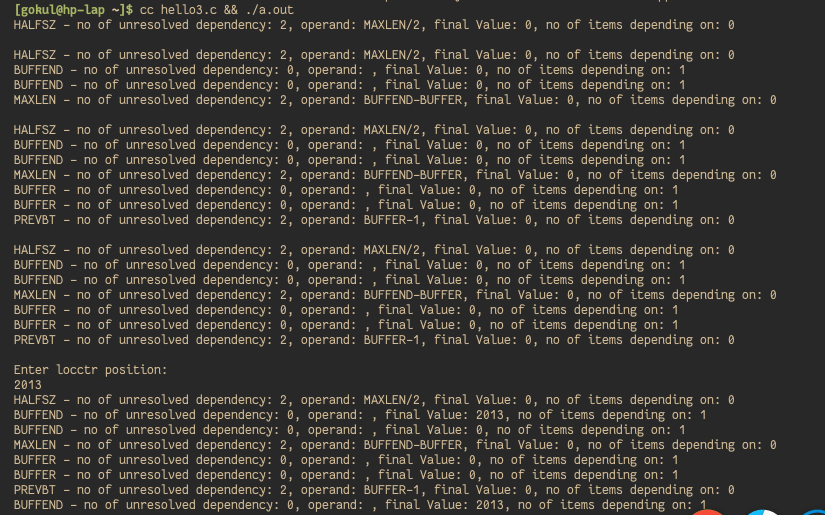
\includegraphics[width=\textwidth]{img/q/ss1.png}

\subsection{Page Replacement}
\subsubsection{Aim}
To implement LRU and FIFO page replacement algorithms
\subsubsection{Algorithms}
\begin{itemize}
    \item LRU \\
    \begin{enumerate}
        \item Read the page reference string
        \item For each entry in page reference string, Check if it exists in frame table
        \item If it does
        \begin{enumerate}
            \item Set the entry in the recently\_used array corresponding to that frame the current index (the position of page in page reference string)
        \end{enumerate}
        \item Else,
        \begin{enumerate}
            \item Find the minimum value of recently used, replace the frame in the corresponding position with incoming page
            \item Set the entry in the recently\_used array corresponding to that frame the current index (the position of page in page reference string)
            \item Increment the number of page faults
        \end{enumerate}
    \end{enumerate}
    \item FIFO \\
    \begin{enumerate}
        \item Read the page reference string
        \item For each entry in page reference string, Check if it exists in frame table
        \item If it does not
        \begin{enumerate}
            \item Replace the frame in the current\_fifo\_idx position with incoming page
            \item Change the current\_fifo\_idx to (current\_fifo\_idx + 1) \% FRAME\_LENGTH
            \item Increment the number of page faults
        \end{enumerate}
    \end{enumerate}
\end{itemize}
\subsubsection{Source Code}
\begin{itemize}
    \item LRU
\end{itemize}
\begin{lstlisting}[language=C]
#include <stdio.h>
#include <stdlib.h>

#define MAX_PAGEREF_LENGTH 25

int find_in_frame(char * frames, int no_of_frames, char query) {
	int i;
	for(i = 0; i < no_of_frames; i++) {
		if(frames[i] == query) return i;
	}

	return -1;
}

int find_min_lru(int * recently_used, int no_of_frames) {
	int min = recently_used[0];
	int min_idx = 0;

	for(int i = 0; i < no_of_frames; i++) {
		if(recently_used[i] <= min) {
			min_idx = i;
			min = recently_used[i];
		}
	}

	return min_idx;
}

int main() {
	int no_of_frames;
	char page_ref_stream[MAX_PAGEREF_LENGTH];
	char * frames;
	int * recently_used;

	int page_faults = 0;
	int lru;

	printf("Enter number of page frames: ");
	scanf("%d%*c", &no_of_frames);

	frames = malloc(sizeof(char) * no_of_frames);
	recently_used = malloc(sizeof(int) * no_of_frames);
	int curr_idx;

	printf("Enter the page reference stream: ");
	scanf("%[^\n]%*c", page_ref_stream);

	for(int i = 0; page_ref_stream[i] != '\0'; i++) {
		if((curr_idx = find_in_frame(
		    frames, no_of_frames, page_ref_stream[i]
		 )) == -1) {
			printf("Page fault for %c\n", 
			    page_ref_stream[i]);
			page_faults++;
			lru = find_min_lru(recently_used, no_of_frames);
			frames[lru] = page_ref_stream[i];
			recently_used[lru] = i+1;
		} else {
			printf("Page hit for %c\n", page_ref_stream[i]);
			recently_used[curr_idx] = i+1;
		}

		printf("Curr frames: ");
		for(int j = 0; j < no_of_frames; j++) 
		    printf("%c ", frames[j]);
		printf("\n");
	}

	printf("\nNumber of page faults = %d\n", page_faults);
	return 0;
}
\end{lstlisting}
\begin{itemize}
    \item FIFO
\end{itemize}
\begin{lstlisting}[language=C]
#include <stdio.h>
#include <stdlib.h>

#define MAX_PAGEREF_LENGTH 25

int find_in_frame(char * frames, int no_of_frames, char query) {
	int i;
	for(i = 0; i < no_of_frames; i++) {
		if(frames[i] == query) return i;
	}

	return -1;
}

int main() {
	int no_of_frames;
	char page_ref_stream[MAX_PAGEREF_LENGTH];
	char * frames;

	int page_faults = 0;
	int fifo_idx = 0;

	printf("Enter number of page frames: ");
	scanf("%d%*c", &no_of_frames);

	frames = malloc(sizeof(char) * no_of_frames);

	printf("Enter the page reference stream: ");
	scanf("%[^\n]%*c", page_ref_stream);

	for(int i = 0; page_ref_stream[i] != '\0'; i++) {
		if(find_in_frame(
		    frames, no_of_frames, page_ref_stream[i]
		) == -1) {
			printf("Page fault for %c\n", 
			    page_ref_stream[i]);
			page_faults++;
			frames[fifo_idx] = page_ref_stream[i];
			fifo_idx = (fifo_idx + 1) % no_of_frames;
		} else {
			printf("Page hit for %c\n", page_ref_stream[i]);
		}


		printf("Curr frames: ");
		for(int j = 0; j < no_of_frames; j++) 
		    printf("%c ", frames[j]);
		printf("\n");
	}

	printf("\nNumber of page faults = %d\n", page_faults);
	return 0;
}
\end{lstlisting}

\subsubsection{Result}
The output of the code is \\
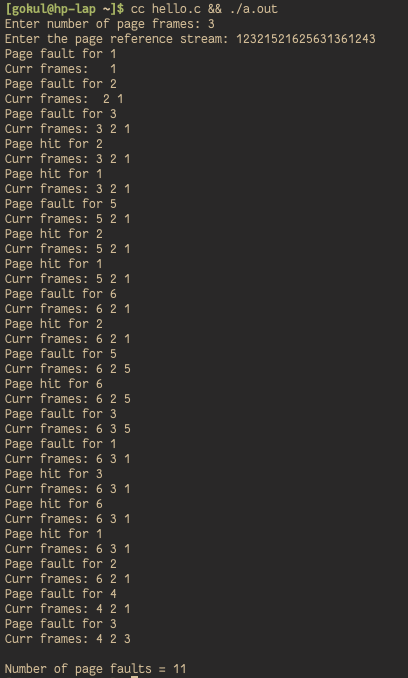
\includegraphics[width=0.9\textwidth]{img/q/ss2.png} \\
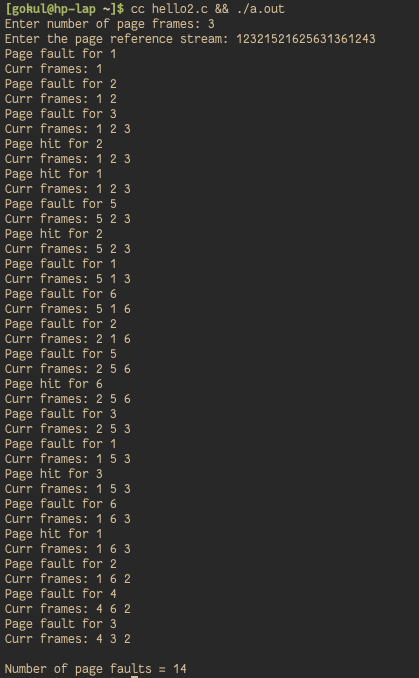
\includegraphics[width=0.9\textwidth]{img/q/ss3.png}

\end{document} 